\chapter{Diagrammes de blocs de définition (bdd)}
\section{Diagramme de bloc générale}
\begin{figure}
	\centering
	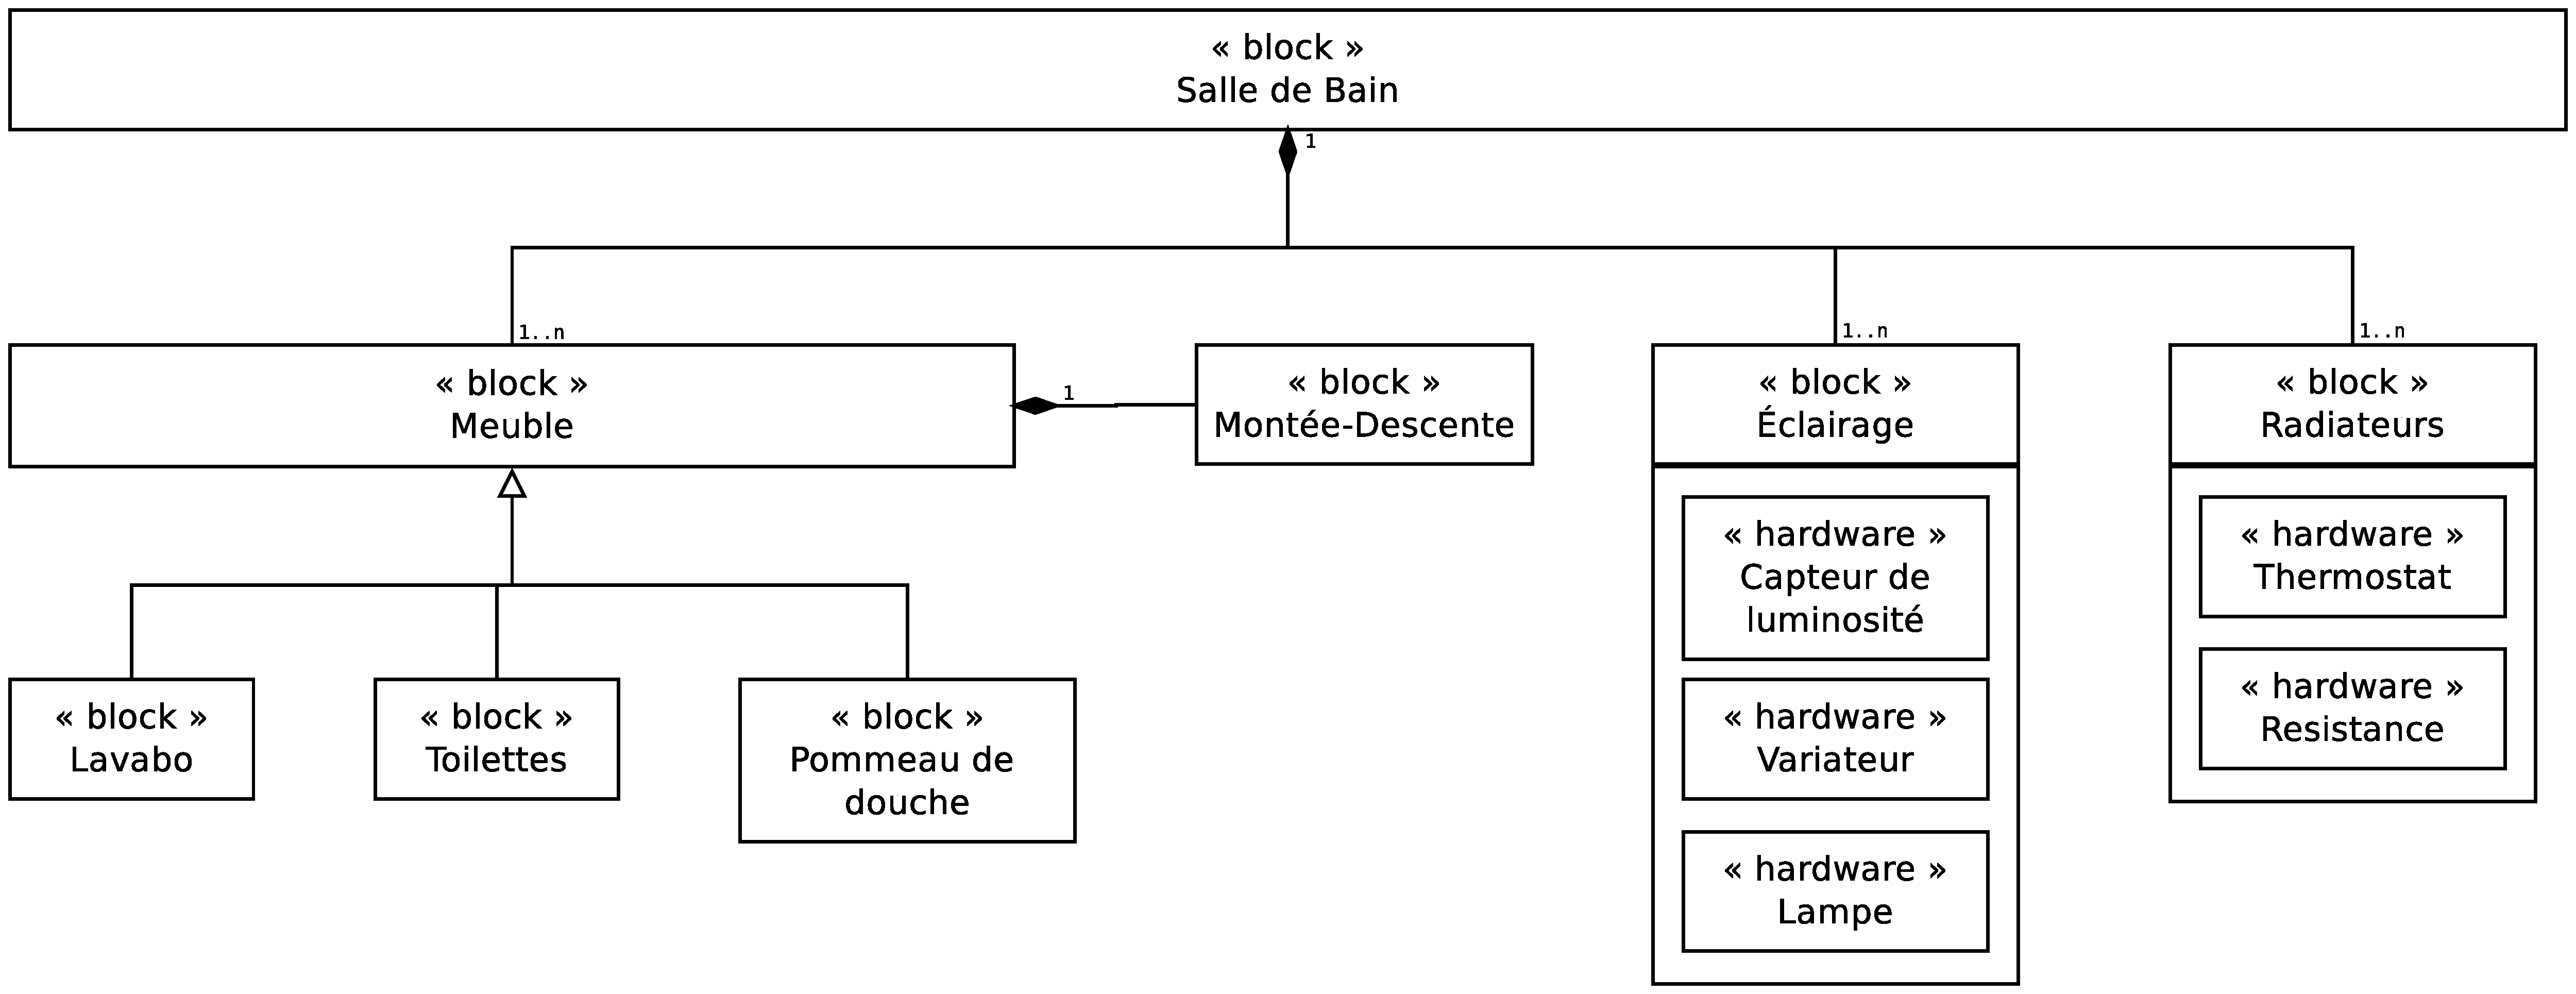
\includegraphics[width=1\linewidth]{diagrams/bathroom/diagramme_blocks_bdd.eps}
	\caption{Diagramme de bloc de définition}
	\label{fig:diagramme_bdd}
\end{figure}

\section{Diagramme de bloc de « Montee-Descente »}
\begin{figure}
	\centering
	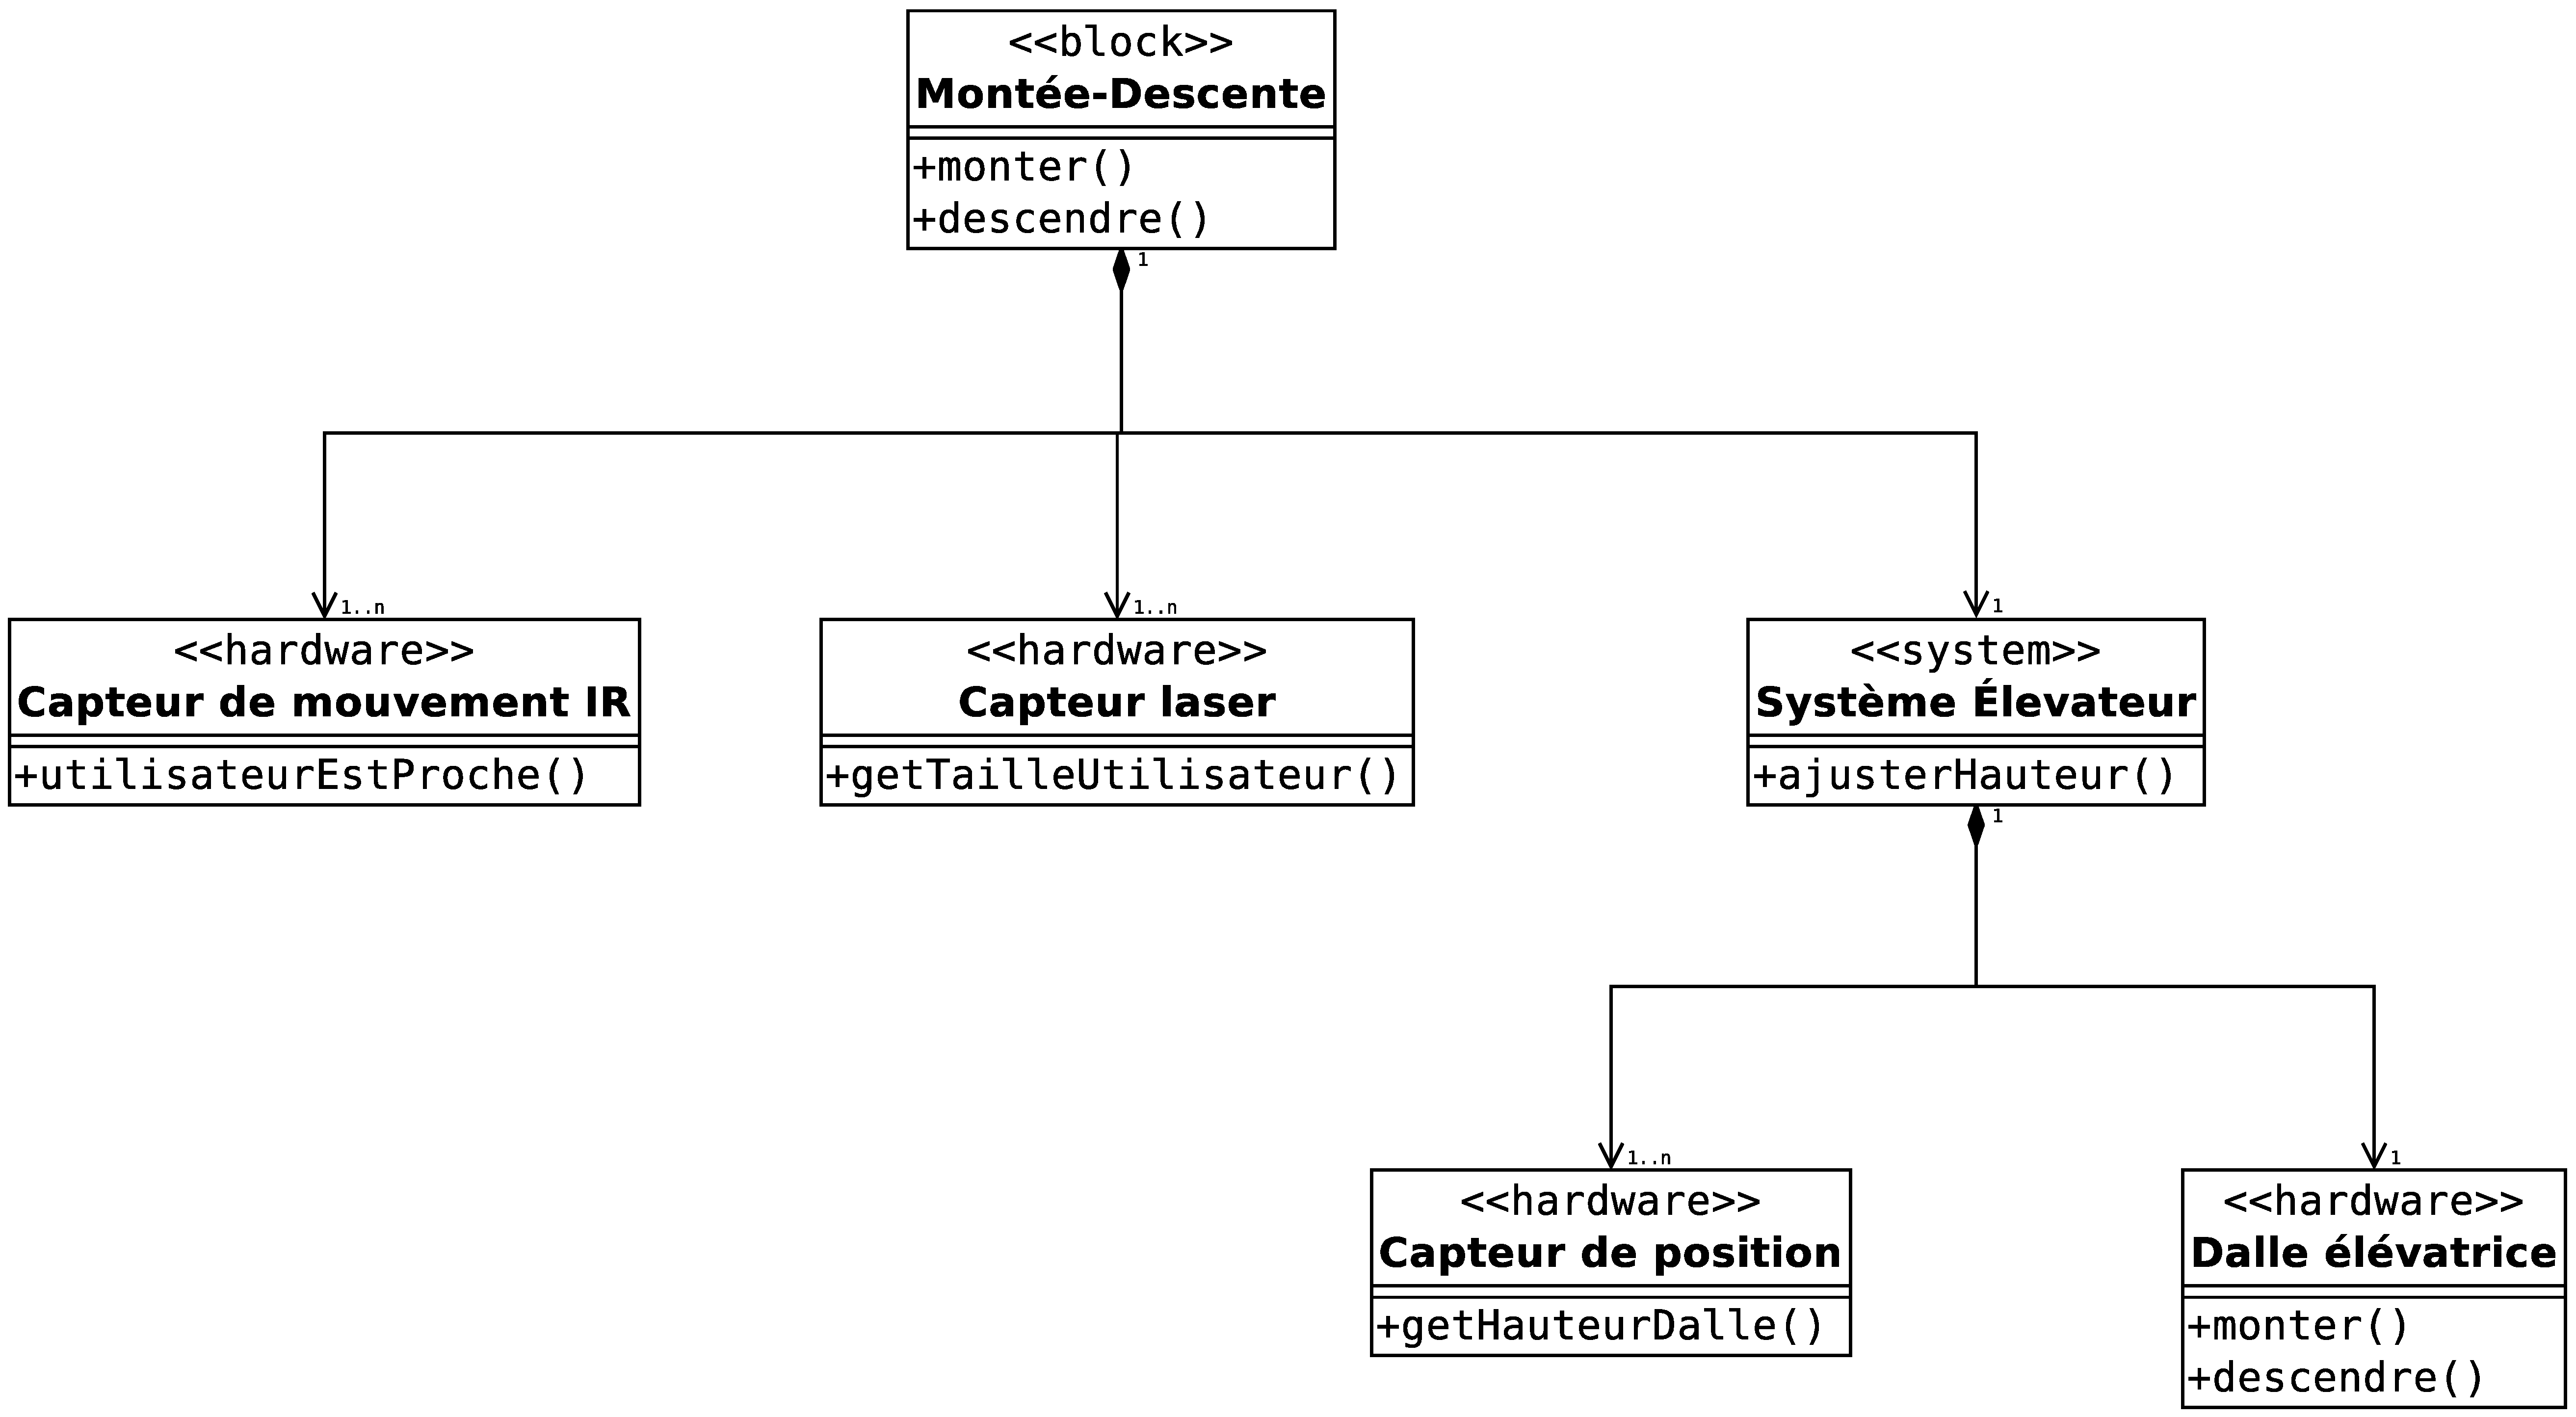
\includegraphics[width=1\linewidth]{diagrams/bathroom/diagramme_blocks_bdd2.eps}
	\caption{Diagramme de bloc de définition de « Montée-Descente »}
	\label{fig:diagramme_bdd2}
\end{figure}

%
%tu penses quoi d'un truc comme ça, ou tu as d'un côté les capteurs utilisés par rapport à l'utilisateur
%et d'un autre le système élevateur avec un capteur de position pour connaitre la hauteur, une dalle élèvatrice et un CPU qui fait les calculs pour savoir comment ajuster la hauteur après elle a dit qu'on doit pas raffiné jusqu'à en crever